%=====================================================================
\section{The charge split in ovals and ellipses}\label{sec:scharge}
\subsection{Accumulated charge: plateau or not}
The accumulated charge $Q(c)$ inside the level $c$ (circle: $c=r$; Cassini: $c=\sqrt{d_1d_2}$; ellipse: scaled copies of the wall)
is the cut-free observable (Sec.~\ref{sec:methods-Q}).
\begin{figure}[H]\centering
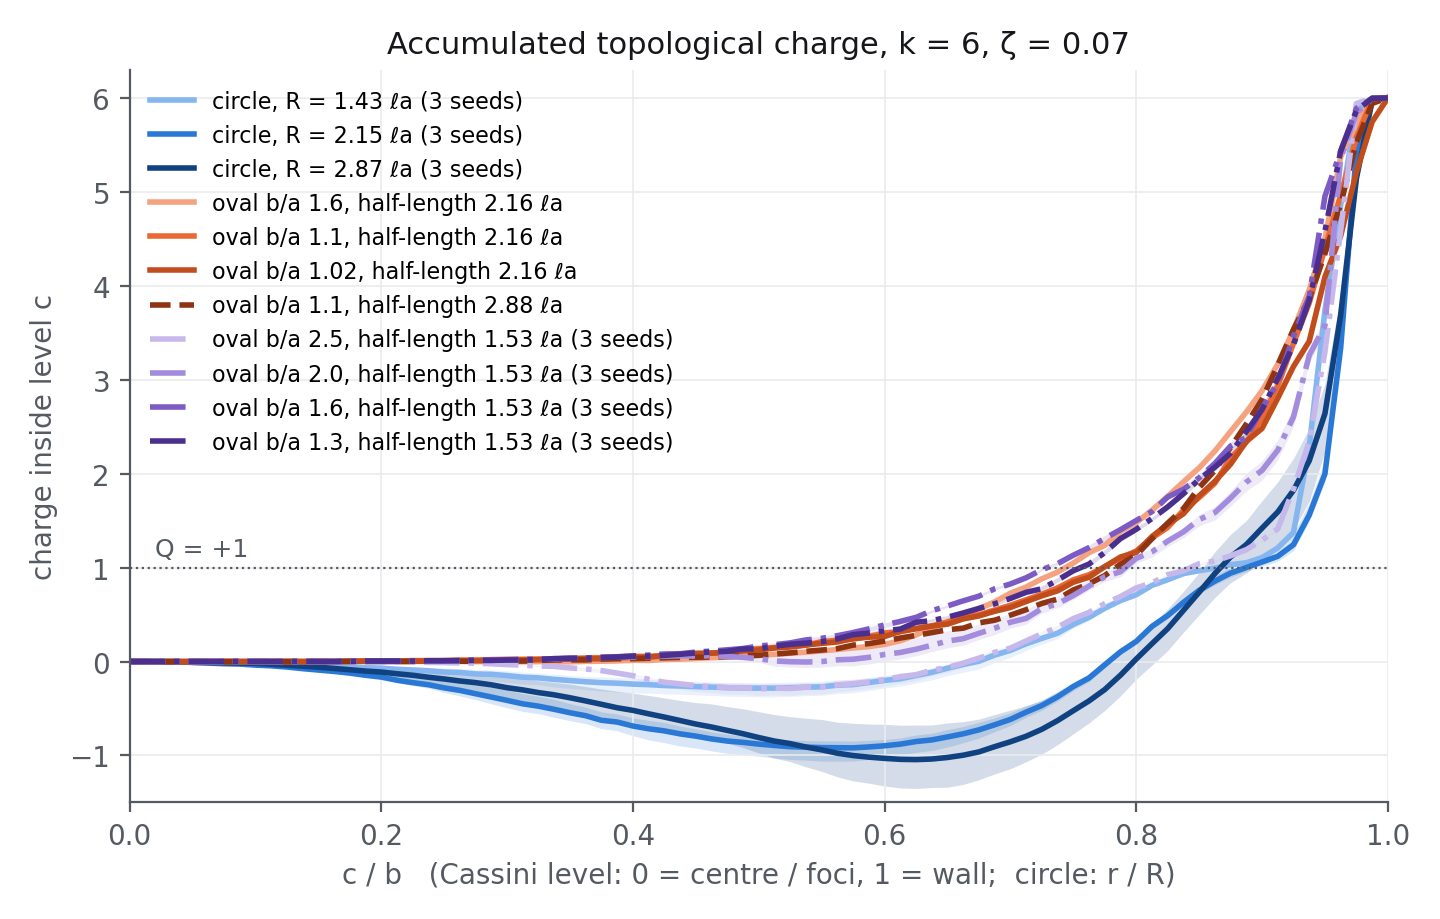
\includegraphics[width=0.85\textwidth]{accumulated_charge.png}
\caption{\textbf{Accumulated charge inside level $c$} ($k=6$, $\zeta=0.07$). Circles (mean of 3 seeds, min--max band): negative
dip ($-\half$ core), plateau at $+1$ for $c/b\approx0.85$--0.93, jump to $k$ within the last few percent (the layer). Ovals of
half-length 2.16 and $2.88\,\la$: monotonic, never negative, no plateau, crossing $+1$ at $c/b\approx0.78$, all on nearly one
curve. Small ovals (half-length $1.53\,\la$, 3 seeds; dash-dotted, light to dark = $b/a$ 2.5 to 1.3): $b/a=2.5$ follows the
circles.}\label{fig:Qc}
\end{figure}

\subsection{Size control: small ovals at half-length $1.53\,\la$}
Four shapes at the size where circles are cleanest, 3 seeds each:
\begin{table}[H]\centering\small
\caption{Small ovals compared with circles of comparable size, all measures. Criteria agree: fraction of $+\half$ on which
mobility and tilt agree with the site rule.}\label{tab:p3}
\begin{adjustbox}{max width=\textwidth}
\begin{tabular}{lccccccc}\toprule
cavity & aspect & sites & $q_b$ (site rule) & labels at wall after 1000 & criteria agree & $d^*/\la$ & $f^*$\\\midrule
circle $R=1.43\,\la$ & 1 & 10 & 1.01--1.05 & 0.87--0.94 & 97--99\% & 0.19--0.20 & 0.26\\
oval $b/a=2.5$ & 1.17 & 10 & 1.07--1.11 & 0.82--0.86 & 97--98\% & 0.22--0.23 & 0.29\\
oval $b/a=2.0$ & 1.29 & 8--9 & 1.6--2.1 & 0.60--0.65 & 81--86\% & 0.29--0.31 & 0.39\\
oval $b/a=1.6$ & 1.51 & (3--7) & 3.3--3.5 & 0.37--0.40 & 72--74\% & 0.41 & 0.53\\
oval $b/a=1.3$ & 1.94 & (3--7) & 3.3--3.6 & 0.42--0.50 & 69--72\% & 0.49--0.50 & 0.63\\\bottomrule
\end{tabular}
\end{adjustbox}
\end{table}
\begin{itemize}
  \item \textbf{Sharp crossover with elongation at fixed size and density:} circle-like at aspect 1.17 ($2k-2$ pinned sites, bulk $+1$,
        wall defects stay), partial at 1.29, lost from $\approx1.4$ while the shape is still convex ($b/a=1.6>\sqrt2$).
  \item In the elongated ovals the site rule finds only a few unstable sites; any cut-free criterion (mobility, tilt or both) gives a
        bulk of 3.1--3.9 (only $\approx4$--5.5 of the 12 imposed $+\half$ behave like wall defects), against 1.1--1.25 in circles of
        the same half-length (Table~\ref{tab:edgeovals}).
\end{itemize}
\begin{table}[H]\centering\small
\caption{Bulk charge $q_b=k-(\text{edge-like})/2$ from the cut-free criteria, $k=6$ (1 seed for the larger ovals).}\label{tab:edgeovals}
\begin{adjustbox}{max width=\textwidth}
\begin{tabular}{lccc}\toprule
cavity & tilted & slow & slow and tilted\\\midrule
circle $1.43\,\la$ (site rule 1.05) & 1.07 & 1.05 & 1.06\\
circle $2.15\,\la$ & 1.11 & 1.25 & 1.24\\
circle $2.87\,\la$ (site rule 1.85) & 1.93 & 2.71 & 2.66\\
ovals half-length $2.16\,\la$, $b/a=1.6$ / 1.1 / 1.02 & 3.42 / 3.58 / 3.26 & 3.66 / 3.44 / 3.10 & 3.85 / 3.87 / 3.57\\
oval half-length $2.88\,\la$, $b/a=1.1$ & 4.03 & 4.25 & 4.45\\\bottomrule
\end{tabular}
\end{adjustbox}
\end{table}
\begin{figure}[H]\centering
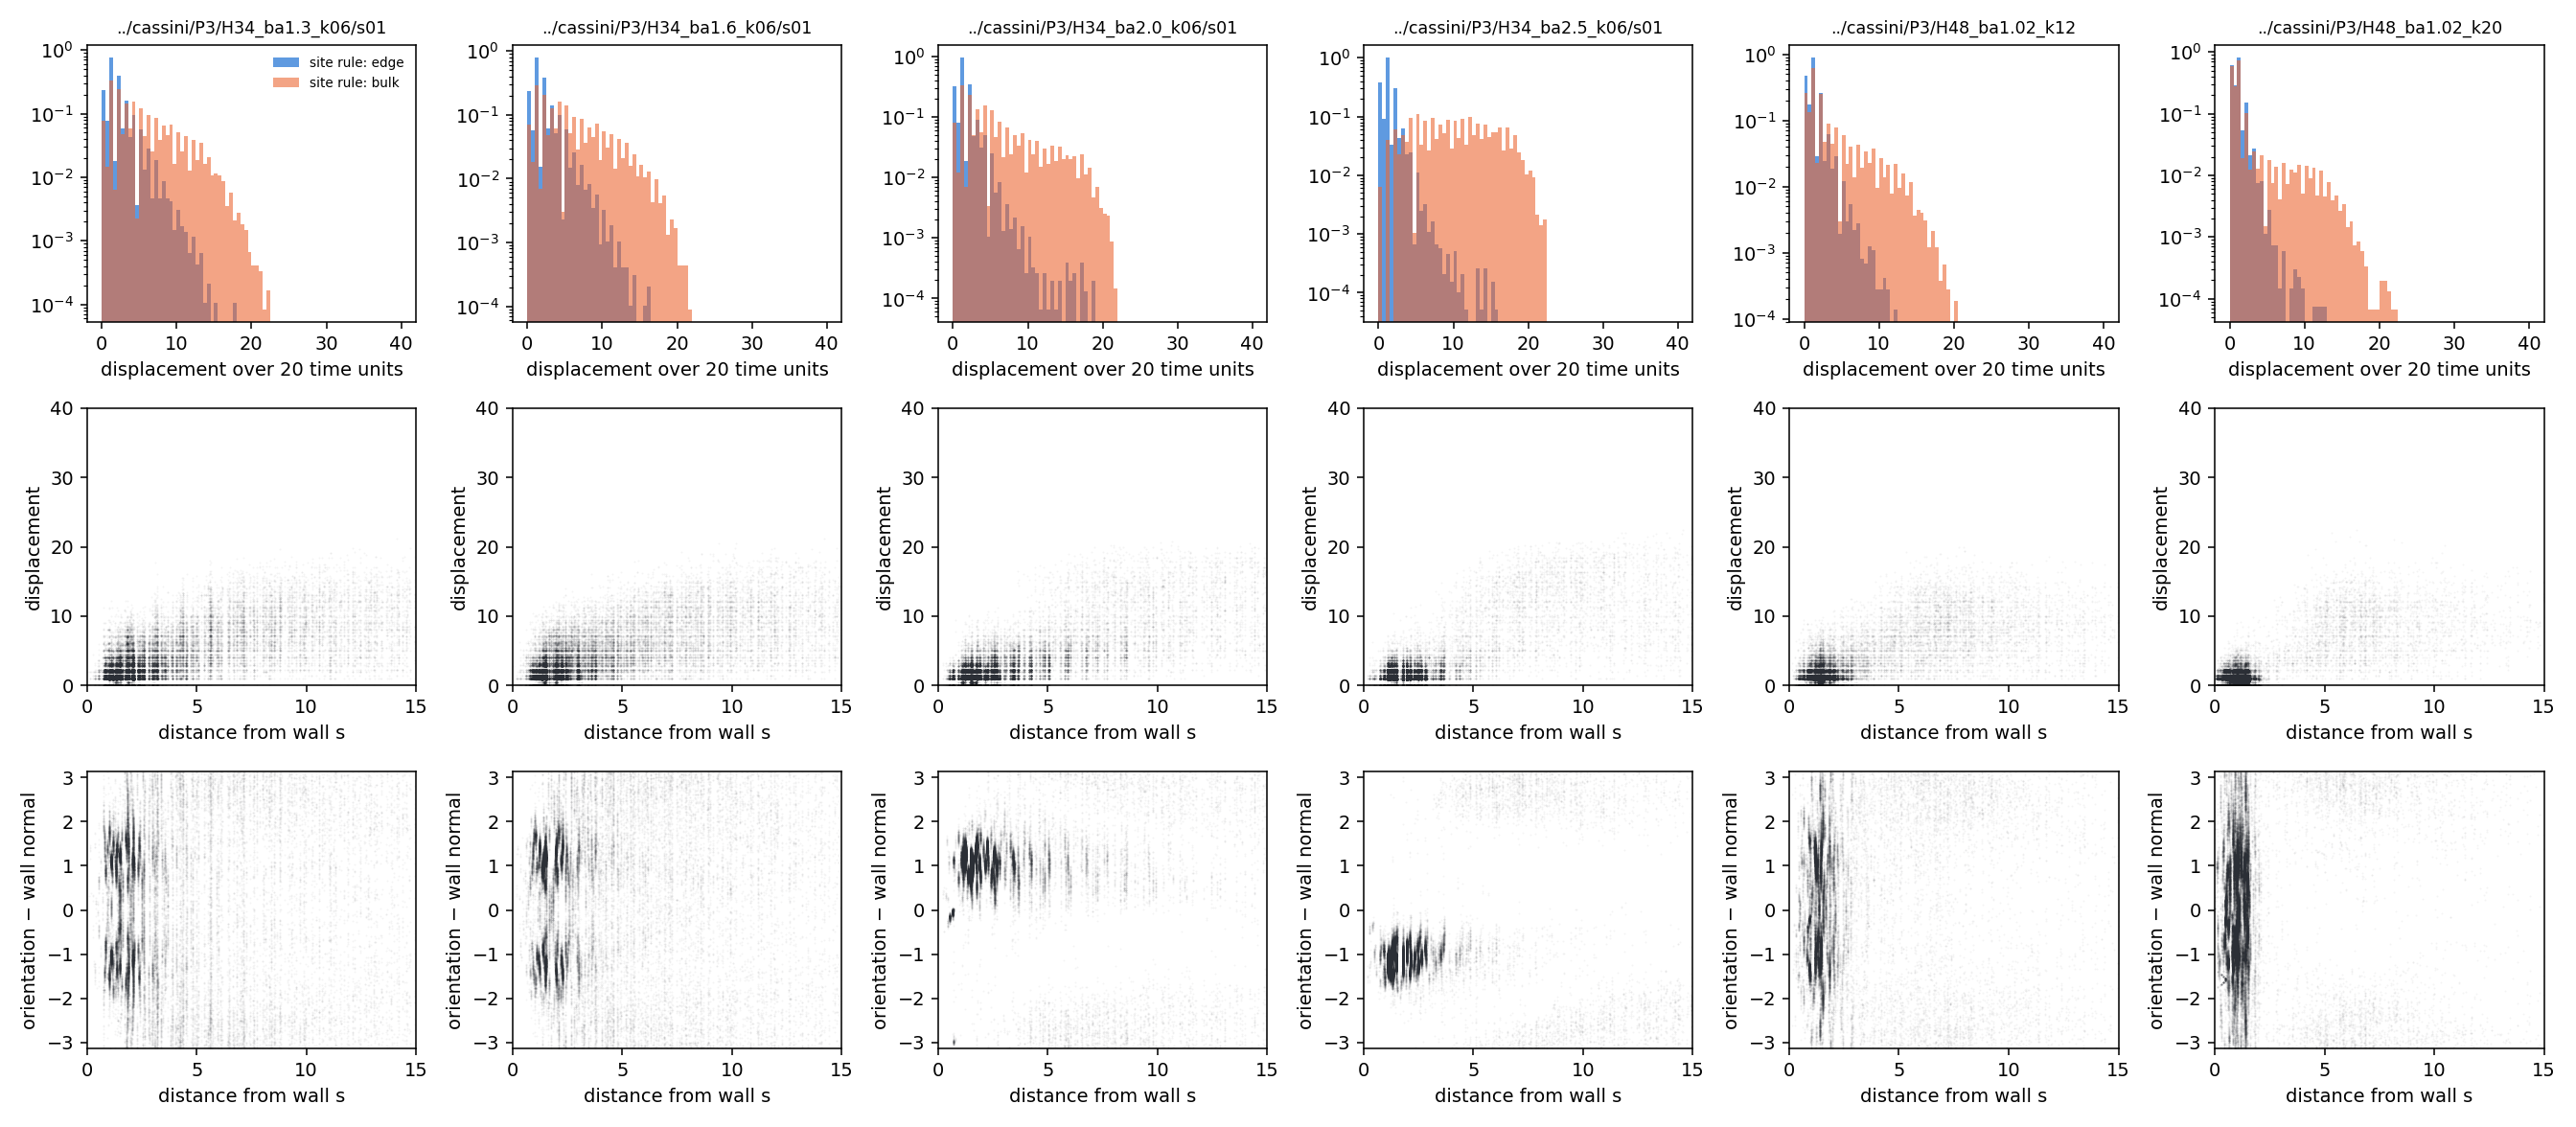
\includegraphics[width=\textwidth]{edge_criteria_small_sel.png}
\caption{Cut-free criteria, seed 1 of each small oval ($b/a=1.3$, 1.6, 2.0, 2.5) and the pinched oval at $k=12$ and 20. Top: displacement over
20 time units (blue: on a site, orange: bulk, by the site rule); middle: displacement against the distance from the wall; bottom:
orientation relative to the outward wall normal against the distance from the wall. Round ovals: wall defects tilted at $\approx\pm1.1$ rad with
one sign (the single vortex). Elongated ovals: both signs, one per lobe vortex. Crowded pinched oval ($k=20$): tilt close to 0, as in
high-density circles. All 16 runs: \texttt{results/6\_shape/small\_ovals\_1.53la/edge\_criteria.png}.}\label{fig:critsmall}
\end{figure}

\subsection{One number per cavity: layer depth $d^*$ and area fraction $f^*$}
$c^*$ = outermost level where $Q$ crosses $+1$; $d^*$ = mean wall distance along that level (circle: $R-c^*$);
$f^*=A(c>c^*)/A$, the fraction of the cavity between the $Q=+1$ level and the wall (Sec.~\ref{sec:methods-dstar}). For a true
layer of fixed width $f^*$ falls as the cavity grows; for charge spread through the cavity $f^*$ is set by the shape alone.
Beyond $f^*=\half$ the ``layer'' would be larger than the bulk it surrounds.
\begin{figure}[H]\centering
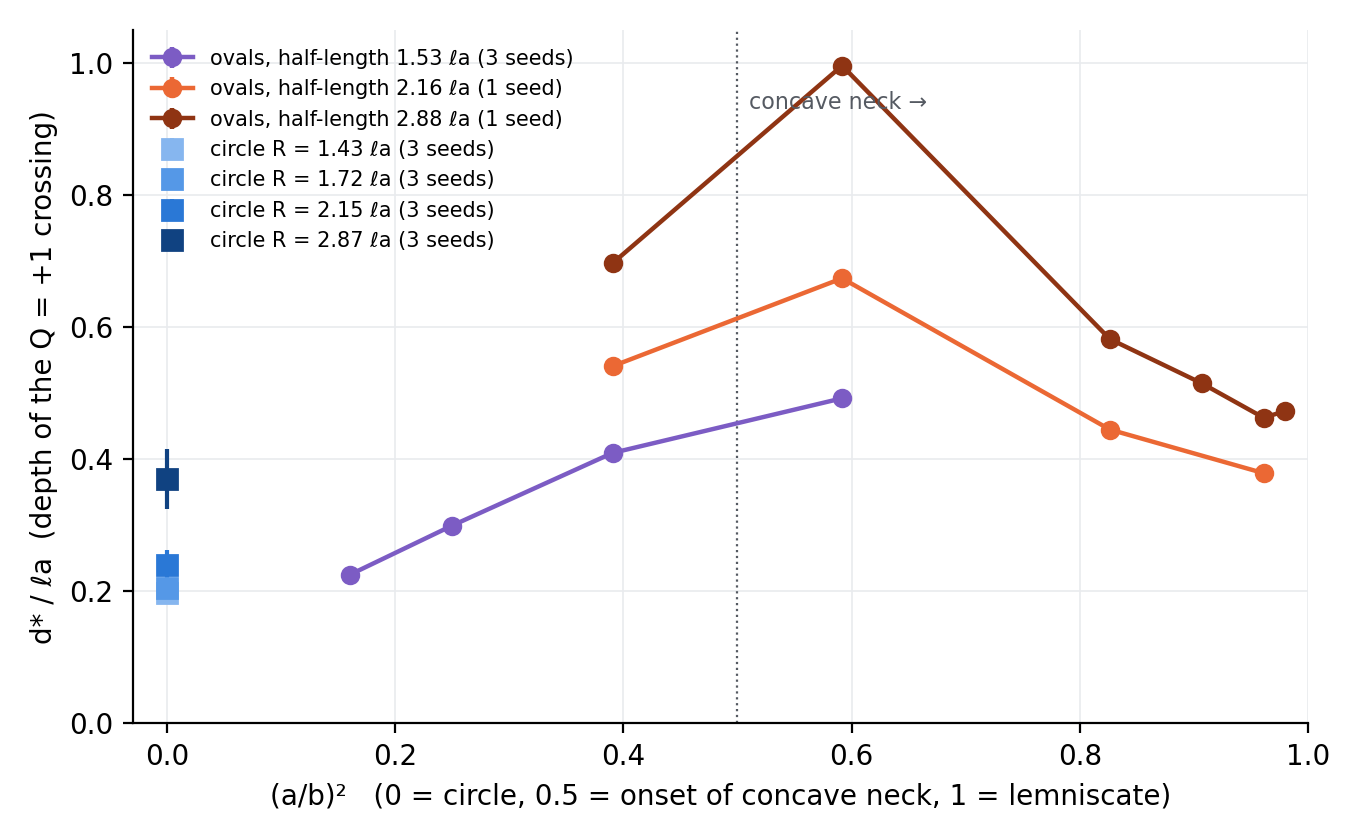
\includegraphics[width=0.82\textwidth]{layer_depth.png}
\caption{Layer depth $d^*/\la$ against elongation $(a/b)^2$ (0 circle, 0.5 onset of the concave neck, 1 lemniscate), $k=6$.
Squares: circles 1.43--$2.87\,\la$. Small ovals (3 seeds) rise from 0.23 to 0.50; larger ovals (1 seed) peak near $b/a\approx1.3$.}\label{fig:dstar}
\end{figure}
\begin{figure}[H]\centering
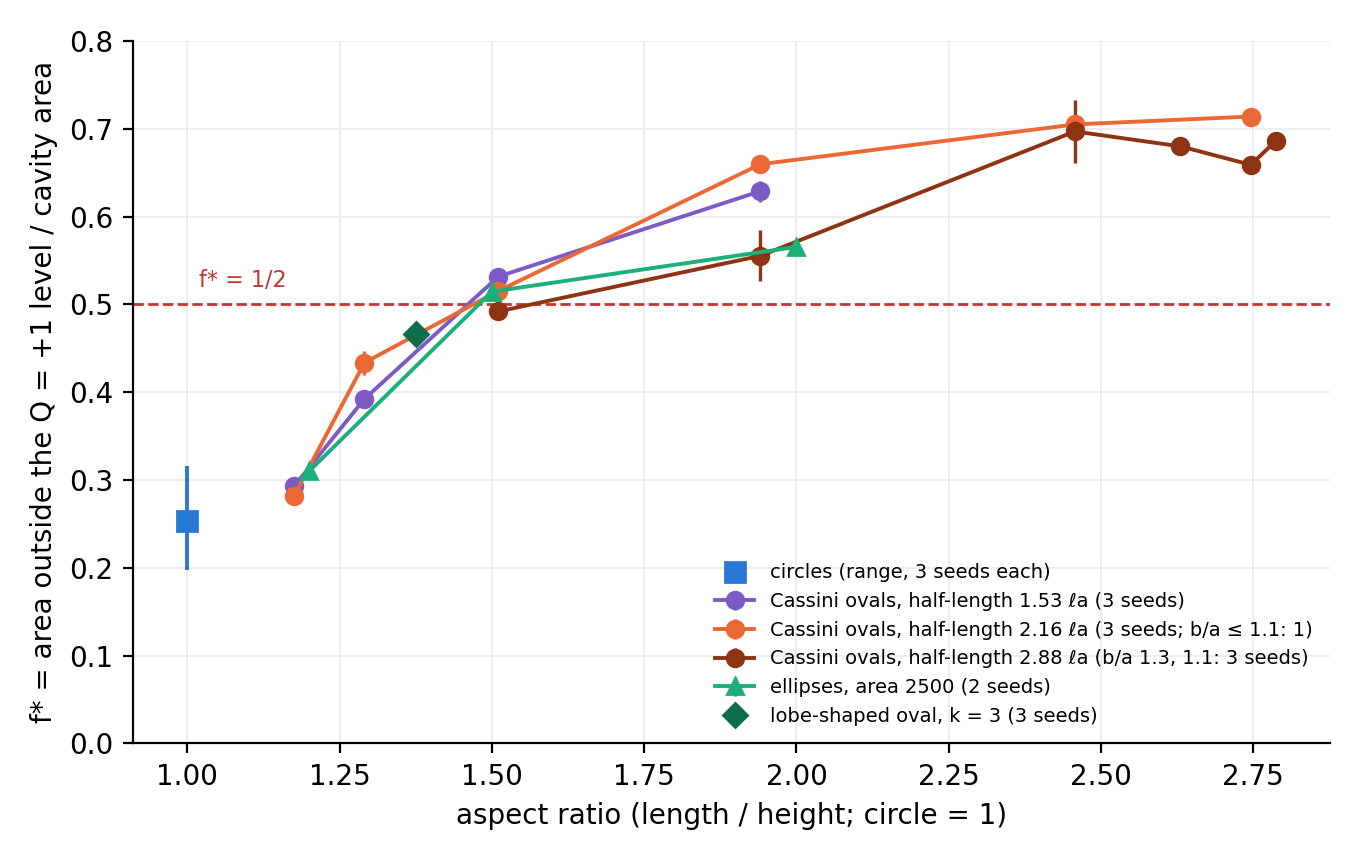
\includegraphics[width=0.85\textwidth]{layer_area_all.png}
\caption{\textbf{Area fraction $f^*$ outside the $Q=+1$ level against the aspect ratio}, all shapes with seeds: Cassini ovals at
three sizes, ellipses (area 2500), the lobe-shaped oval, circles (range over 1.08--$2.15\,\la$, $k=3$ and 6). Dashed: $f^*=\half$.}\label{fig:fstar}
\end{figure}
\begin{itemize}
  \item \textbf{Circles:} $d^*\approx4.5$--6 cells $\approx0.2\,\la$ up to $2.15\,\la$ (0.31--0.42 at $2.87\,\la$); $f^*=0.20$--0.32, falling
        with size (0.26 at 1.43, 0.20 at $2.15\,\la$): a layer of fixed width.
  \item \textbf{Same size, different shape:} at half-length $1.53\,\la$, $d^*/\la=0.23\to0.30\to0.41\to0.50$ for $b/a=2.5\to1.3$.
  \item \textbf{$f^*$ collapses on the aspect ratio for all oval sizes} (half-length 1.53 / 2.16\,$\la$, 3 seeds: $b/a=2.5$: 0.29 / 0.28;
        2.0: 0.39 / 0.42--0.45; 1.6: 0.53 / 0.49--0.54; 1.3: 0.63 / 0.65--0.67), crossing $\half$ near aspect 1.5 and levelling at
        0.65--0.7. At $2.88\,\la$ slightly lower ($\approx0.56$ at aspect 1.94): good but not perfect collapse.
  \item \textbf{Ellipses follow the same curve:} $\varepsilon=1.2$: knee 0.98--1.07, $f^*=0.31$, pinned lattice; 1.5: no knee, $f^*=0.51$--0.52;
        2.0: no knee, $f^*=0.57$ (Table~\ref{tab:ell}). A convex cavity can lose the layer; elongation is the control for both families.
  \item The size independence of $f^*$ is itself the diagnostic of ``no layer''. The equivalent strip width
        $w_\mathrm{eff}=A(c>c^*)/P$ is $0.17$--$0.25\,\la$ for every clean circle layer and grows with size in ovals.
\end{itemize}
\begin{table}[H]\centering\small
\caption{Ellipses (2 seeds): $Q$ at fixed levels, knee and $f^*$.}\label{tab:ell}
\begin{adjustbox}{max width=\textwidth}
\begin{tabular}{lccccc}\toprule
& $Q(0.80)$ & $Q(0.85)$ & $Q(0.90)$ & knee & $f^*$\\\midrule
$\varepsilon=1.2$ & 0.88--0.90 & 1.05--1.07 & 1.32--1.34 & 0.98--1.07 & 0.31\\
$\varepsilon=1.5$ & 1.64--1.68 & 2.10--2.13 & 2.96--2.98 & none & 0.51--0.52\\
$\varepsilon=2.0$ & 1.93--1.95 & 2.46--2.49 & 3.47--3.48 & none & 0.57\\\bottomrule
\end{tabular}
\end{adjustbox}
\end{table}
% NOTE: d* for ellipses is not quoted: layer_depth.py treats an ellipse as a circle of radius R (see Appendix B); f* is unaffected.

\subsection{Not the neck: pinch-off and a lobe-shaped oval}
\begin{itemize}
  \item In the larger ovals $d^*$ falls again as the neck closes ($b/a\to1$). This is \textbf{not} a restored layer: in the tightest necks
        ($b/a=1.01$--1.05) each lobe's charge passes $+1$ about 10 cells from the wall with slope $\mathrm{d}Q/\mathrm{d}(c/b)\approx8$--10
        (circle plateau $\approx3$, circle layer jump 50--100), the whole cavity passes $+2$ without a plateau, and $Q_L\approx Q_R$. The
        lobes are just smaller.
  \item Circles with the area of one lobe and half the winding ($k=3$, $R=1.08$ and $1.43\,\la$, 3 seeds) keep a normal layer
        ($d^*=4.1$--5.0 cells, $+1$ plateau). A lobe does not behave like a circle of its size, even with a 13-cell neck.
  \item \textbf{A single convex oval with the area and aspect of one lobe} ($b/a=1.8$, aspect 1.38, $k=3$, 3 seeds) loses the layer too:
        3 sites instead of $2k-2=4$, $q_b\approx1.9$ of 3, $d^*/\la=0.31$--0.32 (circles of the same area 0.18--0.22), $Q(c)$ smooth,
        only 16--28\% of the wall labels at the wall after 1000. The lobe shape is enough; no coupling through the neck is needed.
\end{itemize}

\subsection{The winding: crowded walls push back}
\begin{table}[H]\centering\small
\caption{$k$ scan at half-length $1.53\,\la$ (3 seeds): $Q$ at the fixed level $c/b=0.85$ (no knee needed); in brackets the knees
found (seeds) and their value.}\label{tab:kscan}
\begin{adjustbox}{max width=\textwidth}
\begin{tabular}{lcccccc}\toprule
& $k=2$ & 4 & 6 & 8 & 10 & 12\\\midrule
circle $R=1.43\,\la$ & 0.99 & 0.95 & 0.95 & 0.94 & 0.97 & --\\
oval $b/a=2.0$ & 1.12 & 1.54 & 1.51 & 1.49 & 1.36 & 1.24 (3/3, 1.31)\\
oval $b/a=1.6$ & 1.30 & 2.06 & 1.96 & 1.63 & 1.42 (1/3, 1.54) & 1.31 (3/3, 1.40)\\\bottomrule
\end{tabular}
\end{adjustbox}
\end{table}
\begin{figure}[H]\centering
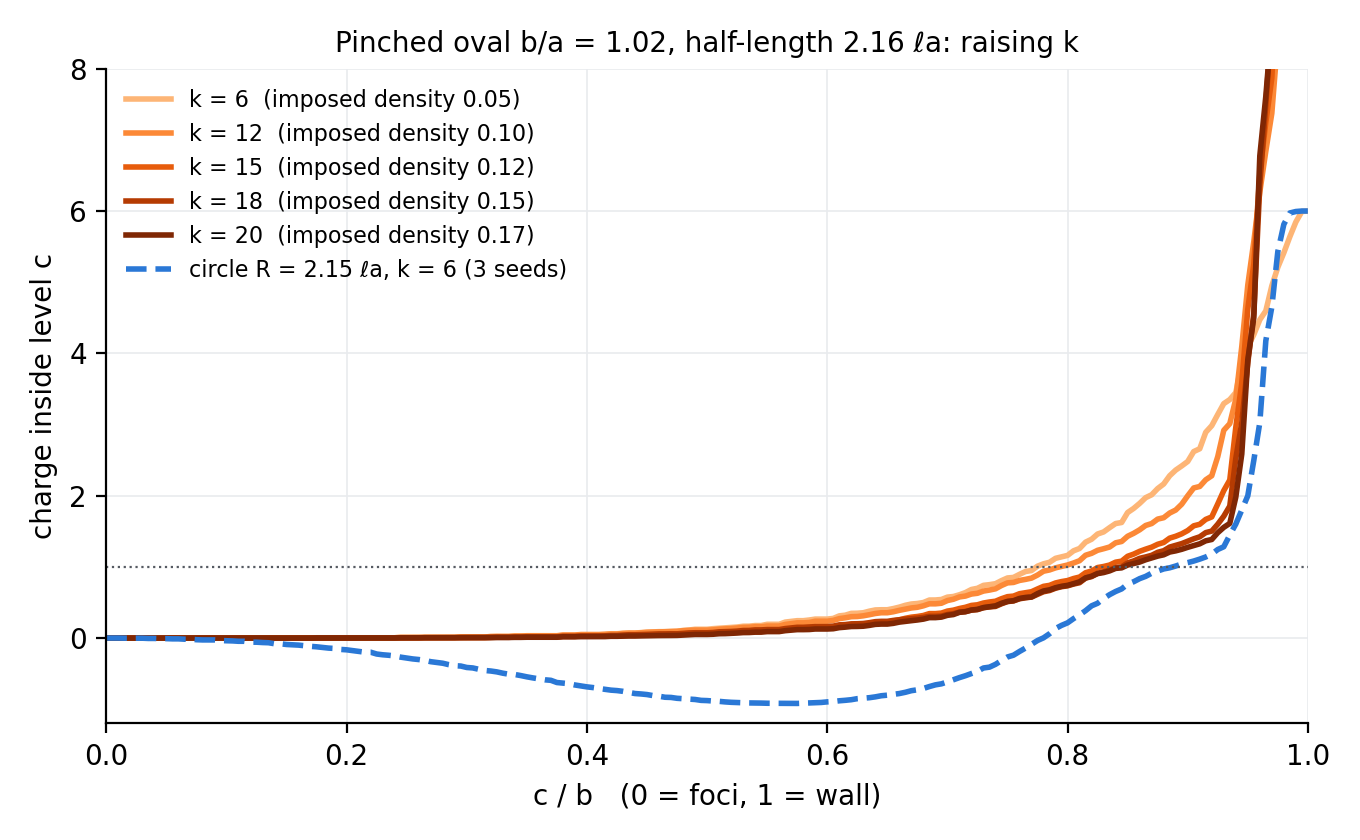
\includegraphics[width=0.82\textwidth]{highk.png}
\caption{Accumulated charge in the pinched oval ($b/a=1.02$, half-length $2.16\,\la$) for $k=6$ to 20 (imposed density 0.05 to 0.17), with
the circle of $R=2.15\,\la$ for reference.}\label{fig:highk}
\end{figure}
\begin{itemize}
  \item \textbf{Circle: a traditional layer}, $Q$ at fixed depth independent of $k$ (slope $-0.002$ per unit $k$): all extra winding goes
        to the wall.
  \item \textbf{Ovals: a bounded, non-monotonic excess.} The bulk carries at most $\approx+1$ extra at moderate $k$ ($\rho\approx0.04$--0.07),
        and the excess shrinks again as the wall gets crowded; at $k=12$ ($\rho\approx0.13$) a plateau and a wall lattice reappear
        ($f_\mathrm{static}$ for $b/a=1.6$: 0.03, 0.21, 0.11, 0.39, 0.70 for $k=2\dots12$, 1 seed).
  \item \textbf{Pinched oval at high $k$:} $Q(c/b=0.85)$ falls from 1.76 ($k=6$) to 1.03--1.06 ($k=18$, 20), $d^*/\la$ from 0.38 to 0.30
        (circle 0.20), labels stay at the wall (84\% after 1000 at $k=15$, 18). The bulk carries $\approx+1$ \emph{for the whole cavity},
        $\approx+\half$ per lobe, not $+1$ per lobe. 1 seed; $k=18$--20 at the edge of the anchoring resolution.
  \item Same trend as the mirror runs (Sec.~\ref{sec:mirror}): \textbf{a crowded wall favours the topological structure}; elongation
        matters most at moderate imposed density.
\end{itemize}
